\documentclass[]{article}
\usepackage{lmodern}
\usepackage{amssymb,amsmath}
\usepackage{ifxetex,ifluatex}
\usepackage{fixltx2e} % provides \textsubscript
\ifnum 0\ifxetex 1\fi\ifluatex 1\fi=0 % if pdftex
  \usepackage[T1]{fontenc}
  \usepackage[utf8]{inputenc}
\else % if luatex or xelatex
  \ifxetex
    \usepackage{mathspec}
  \else
    \usepackage{fontspec}
  \fi
  \defaultfontfeatures{Ligatures=TeX,Scale=MatchLowercase}
\fi
% use upquote if available, for straight quotes in verbatim environments
\IfFileExists{upquote.sty}{\usepackage{upquote}}{}
% use microtype if available
\IfFileExists{microtype.sty}{%
\usepackage{microtype}
\UseMicrotypeSet[protrusion]{basicmath} % disable protrusion for tt fonts
}{}
\usepackage[margin=1in]{geometry}
\usepackage{hyperref}
\hypersetup{unicode=true,
            pdftitle={hw1},
            pdfauthor={Kevin Luo},
            pdfborder={0 0 0},
            breaklinks=true}
\urlstyle{same}  % don't use monospace font for urls
\usepackage{color}
\usepackage{fancyvrb}
\newcommand{\VerbBar}{|}
\newcommand{\VERB}{\Verb[commandchars=\\\{\}]}
\DefineVerbatimEnvironment{Highlighting}{Verbatim}{commandchars=\\\{\}}
% Add ',fontsize=\small' for more characters per line
\usepackage{framed}
\definecolor{shadecolor}{RGB}{248,248,248}
\newenvironment{Shaded}{\begin{snugshade}}{\end{snugshade}}
\newcommand{\KeywordTok}[1]{\textcolor[rgb]{0.13,0.29,0.53}{\textbf{#1}}}
\newcommand{\DataTypeTok}[1]{\textcolor[rgb]{0.13,0.29,0.53}{#1}}
\newcommand{\DecValTok}[1]{\textcolor[rgb]{0.00,0.00,0.81}{#1}}
\newcommand{\BaseNTok}[1]{\textcolor[rgb]{0.00,0.00,0.81}{#1}}
\newcommand{\FloatTok}[1]{\textcolor[rgb]{0.00,0.00,0.81}{#1}}
\newcommand{\ConstantTok}[1]{\textcolor[rgb]{0.00,0.00,0.00}{#1}}
\newcommand{\CharTok}[1]{\textcolor[rgb]{0.31,0.60,0.02}{#1}}
\newcommand{\SpecialCharTok}[1]{\textcolor[rgb]{0.00,0.00,0.00}{#1}}
\newcommand{\StringTok}[1]{\textcolor[rgb]{0.31,0.60,0.02}{#1}}
\newcommand{\VerbatimStringTok}[1]{\textcolor[rgb]{0.31,0.60,0.02}{#1}}
\newcommand{\SpecialStringTok}[1]{\textcolor[rgb]{0.31,0.60,0.02}{#1}}
\newcommand{\ImportTok}[1]{#1}
\newcommand{\CommentTok}[1]{\textcolor[rgb]{0.56,0.35,0.01}{\textit{#1}}}
\newcommand{\DocumentationTok}[1]{\textcolor[rgb]{0.56,0.35,0.01}{\textbf{\textit{#1}}}}
\newcommand{\AnnotationTok}[1]{\textcolor[rgb]{0.56,0.35,0.01}{\textbf{\textit{#1}}}}
\newcommand{\CommentVarTok}[1]{\textcolor[rgb]{0.56,0.35,0.01}{\textbf{\textit{#1}}}}
\newcommand{\OtherTok}[1]{\textcolor[rgb]{0.56,0.35,0.01}{#1}}
\newcommand{\FunctionTok}[1]{\textcolor[rgb]{0.00,0.00,0.00}{#1}}
\newcommand{\VariableTok}[1]{\textcolor[rgb]{0.00,0.00,0.00}{#1}}
\newcommand{\ControlFlowTok}[1]{\textcolor[rgb]{0.13,0.29,0.53}{\textbf{#1}}}
\newcommand{\OperatorTok}[1]{\textcolor[rgb]{0.81,0.36,0.00}{\textbf{#1}}}
\newcommand{\BuiltInTok}[1]{#1}
\newcommand{\ExtensionTok}[1]{#1}
\newcommand{\PreprocessorTok}[1]{\textcolor[rgb]{0.56,0.35,0.01}{\textit{#1}}}
\newcommand{\AttributeTok}[1]{\textcolor[rgb]{0.77,0.63,0.00}{#1}}
\newcommand{\RegionMarkerTok}[1]{#1}
\newcommand{\InformationTok}[1]{\textcolor[rgb]{0.56,0.35,0.01}{\textbf{\textit{#1}}}}
\newcommand{\WarningTok}[1]{\textcolor[rgb]{0.56,0.35,0.01}{\textbf{\textit{#1}}}}
\newcommand{\AlertTok}[1]{\textcolor[rgb]{0.94,0.16,0.16}{#1}}
\newcommand{\ErrorTok}[1]{\textcolor[rgb]{0.64,0.00,0.00}{\textbf{#1}}}
\newcommand{\NormalTok}[1]{#1}
\usepackage{graphicx,grffile}
\makeatletter
\def\maxwidth{\ifdim\Gin@nat@width>\linewidth\linewidth\else\Gin@nat@width\fi}
\def\maxheight{\ifdim\Gin@nat@height>\textheight\textheight\else\Gin@nat@height\fi}
\makeatother
% Scale images if necessary, so that they will not overflow the page
% margins by default, and it is still possible to overwrite the defaults
% using explicit options in \includegraphics[width, height, ...]{}
\setkeys{Gin}{width=\maxwidth,height=\maxheight,keepaspectratio}
\IfFileExists{parskip.sty}{%
\usepackage{parskip}
}{% else
\setlength{\parindent}{0pt}
\setlength{\parskip}{6pt plus 2pt minus 1pt}
}
\setlength{\emergencystretch}{3em}  % prevent overfull lines
\providecommand{\tightlist}{%
  \setlength{\itemsep}{0pt}\setlength{\parskip}{0pt}}
\setcounter{secnumdepth}{0}
% Redefines (sub)paragraphs to behave more like sections
\ifx\paragraph\undefined\else
\let\oldparagraph\paragraph
\renewcommand{\paragraph}[1]{\oldparagraph{#1}\mbox{}}
\fi
\ifx\subparagraph\undefined\else
\let\oldsubparagraph\subparagraph
\renewcommand{\subparagraph}[1]{\oldsubparagraph{#1}\mbox{}}
\fi

%%% Use protect on footnotes to avoid problems with footnotes in titles
\let\rmarkdownfootnote\footnote%
\def\footnote{\protect\rmarkdownfootnote}

%%% Change title format to be more compact
\usepackage{titling}

% Create subtitle command for use in maketitle
\providecommand{\subtitle}[1]{
  \posttitle{
    \begin{center}\large#1\end{center}
    }
}

\setlength{\droptitle}{-2em}

  \title{hw1}
    \pretitle{\vspace{\droptitle}\centering\huge}
  \posttitle{\par}
    \author{Kevin Luo}
    \preauthor{\centering\large\emph}
  \postauthor{\par}
      \predate{\centering\large\emph}
  \postdate{\par}
    \date{2019/9/11}


\begin{document}
\maketitle

\section*{1. Specification searches}\subsubsection*{1.1 Data Prep}

\begin{Shaded}
\begin{Highlighting}[]
\NormalTok{dat <-}\StringTok{ }\KeywordTok{read.table}\NormalTok{(}\StringTok{"cps1re74.csv"}\NormalTok{,}\DataTypeTok{header=}\NormalTok{T)}
\CommentTok{# unemployed}
\NormalTok{dat}\OperatorTok{$}\NormalTok{u74 <-}\StringTok{ }\KeywordTok{as.numeric}\NormalTok{(dat}\OperatorTok{$}\NormalTok{re74}\OperatorTok{==}\DecValTok{0}\NormalTok{)}
\NormalTok{dat}\OperatorTok{$}\NormalTok{u75 <-}\StringTok{ }\KeywordTok{as.numeric}\NormalTok{(dat}\OperatorTok{$}\NormalTok{re75}\OperatorTok{==}\DecValTok{0}\NormalTok{)}
\NormalTok{## linear regression on the outcome}
\NormalTok{lmoutcome =}\StringTok{ }\KeywordTok{lm}\NormalTok{(re78 }\OperatorTok{~}\StringTok{ }\NormalTok{., }\DataTypeTok{data =}\NormalTok{ dat)}
\NormalTok{lmoutcome}\OperatorTok{$}\NormalTok{coefficients[}\StringTok{'treat'}\NormalTok{]}
\end{Highlighting}
\end{Shaded}

\begin{verbatim}
##    treat 
## 1067.546
\end{verbatim}

\begin{Shaded}
\begin{Highlighting}[]
\NormalTok{lmoutcome =}\StringTok{ }\KeywordTok{lm}\NormalTok{(re78 }\OperatorTok{~}\StringTok{ }\NormalTok{treat, }\DataTypeTok{data =}\NormalTok{ dat)}
\end{Highlighting}
\end{Shaded}

\subsubsection*{1.2 Function Design}

Run 1024 linear regressions with subsets of covariates, and report the
regression coefficients of the treatment. How many are positively
significant, how many are negatively significant, and how many are not
significant?

\begin{Shaded}
\begin{Highlighting}[]
\NormalTok{alpha <-}\StringTok{ }\FloatTok{0.05}
\NormalTok{positive <-}\StringTok{ }\DecValTok{0}
\NormalTok{negative <-}\StringTok{ }\DecValTok{0}
\NormalTok{R2 <-}\StringTok{ }\KeywordTok{rep}\NormalTok{(}\DecValTok{0}\NormalTok{,}\DecValTok{1024}\NormalTok{)}

\CommentTok{# filter the dependent variable and treatment to ensure the 1-1 mapping}
\CommentTok{# between our index and the variable}
\NormalTok{ind_dat <-}\StringTok{ }\NormalTok{dat }\OperatorTok
\StringTok{  }\KeywordTok{select}\NormalTok{(}\OperatorTok{-}\StringTok{"re78"}\NormalTok{, }\OperatorTok{-}\StringTok{"treat"}\NormalTok{)}

\CommentTok{# The main idea here is to use bit-operation to perform the loop.}
\CommentTok{# For each variable j, the index we created in listI[[1]][j] }
\CommentTok{# determined whether it shall be included in our lm.}
\CommentTok{# Besides the statistical inference of the coefficient, we also report R^2}
\ControlFlowTok{for}\NormalTok{ (i }\ControlFlowTok{in} \DecValTok{0}\OperatorTok{:}\DecValTok{1023}\NormalTok{)\{}
\NormalTok{  binaryI <-}\StringTok{ }\KeywordTok{intToBin}\NormalTok{(i)}
\NormalTok{  strI <-}\StringTok{ }\KeywordTok{as.character}\NormalTok{(binaryI)}
\NormalTok{  listI <-}\StringTok{ }\KeywordTok{strsplit}\NormalTok{(strI, }\StringTok{""}\NormalTok{)}
\NormalTok{  modelSpecification <-}\StringTok{ "re78 ~ treat"}
  
  \CommentTok{# The model specification is hence decided and updated}
  \CommentTok{# according to the different values of i}
  \ControlFlowTok{for}\NormalTok{ (j }\ControlFlowTok{in} \DecValTok{1}\OperatorTok{:}\KeywordTok{nchar}\NormalTok{(strI))\{}
    \ControlFlowTok{if}\NormalTok{ (listI[[}\DecValTok{1}\NormalTok{]][j] }\OperatorTok{==}\StringTok{ "1"}\NormalTok{)\{}
\NormalTok{      modelSpecification <-}\StringTok{ }\KeywordTok{paste}\NormalTok{(modelSpecification, }\StringTok{"+"}\NormalTok{, }\KeywordTok{colnames}\NormalTok{(ind_dat)[j])}
\NormalTok{    \}}
\NormalTok{  \}}
\NormalTok{  lmtemp <-}\StringTok{ }\KeywordTok{lm}\NormalTok{(modelSpecification, }\DataTypeTok{data =}\NormalTok{ dat)}
\NormalTok{  R2[i}\OperatorTok{+}\DecValTok{1}\NormalTok{] <-}\StringTok{ }\KeywordTok{as.numeric}\NormalTok{(}\KeywordTok{summary}\NormalTok{(lmtemp)[}\StringTok{'r.squared'}\NormalTok{])}
  \ControlFlowTok{if}\NormalTok{ (}\KeywordTok{summary}\NormalTok{(lmtemp)}\OperatorTok{$}\NormalTok{coefficients[}\StringTok{'treat'}\NormalTok{,}\StringTok{'Pr(>|t|)'}\NormalTok{] }\OperatorTok{<}\StringTok{ }\NormalTok{alpha }
      \OperatorTok{&}\StringTok{ }\NormalTok{lmtemp}\OperatorTok{$}\NormalTok{coefficients[}\StringTok{'treat'}\NormalTok{] }\OperatorTok{>}\StringTok{ }\DecValTok{0}\NormalTok{)\{}
\NormalTok{    positive <-}\StringTok{ }\NormalTok{positive }\OperatorTok{+}\StringTok{ }\DecValTok{1}
\NormalTok{  \}}
  \ControlFlowTok{if}\NormalTok{ (}\KeywordTok{summary}\NormalTok{(lmtemp)}\OperatorTok{$}\NormalTok{coefficients[}\StringTok{'treat'}\NormalTok{,}\StringTok{'Pr(>|t|)'}\NormalTok{] }\OperatorTok{<}\StringTok{ }\NormalTok{alpha }
      \OperatorTok{&}\StringTok{ }\NormalTok{lmtemp}\OperatorTok{$}\NormalTok{coefficients[}\StringTok{'treat'}\NormalTok{] }\OperatorTok{<}\StringTok{ }\DecValTok{0}\NormalTok{)\{}
\NormalTok{    negative <-}\StringTok{ }\NormalTok{negative }\OperatorTok{+}\StringTok{ }\DecValTok{1}
\NormalTok{  \}}
\NormalTok{\}}
\NormalTok{negative}
\end{Highlighting}
\end{Shaded}

\begin{verbatim}
## [1] 198
\end{verbatim}

\begin{Shaded}
\begin{Highlighting}[]
\NormalTok{positive}
\end{Highlighting}
\end{Shaded}

\begin{verbatim}
## [1] 125
\end{verbatim}

There're 198 negative significant coefficients of treatment and 125
positive ones.

\begin{Shaded}
\begin{Highlighting}[]
\CommentTok{# Also some interesting results concerning the choice of parameters.}
\NormalTok{R2<-}\StringTok{ }\KeywordTok{as.data.frame}\NormalTok{(R2)}
\NormalTok{R2 }\OperatorTok
\StringTok{  }\KeywordTok{mutate}\NormalTok{(}\DataTypeTok{index =} \DecValTok{1}\OperatorTok{:}\KeywordTok{length}\NormalTok{(R2)) }\OperatorTok
\StringTok{  }\KeywordTok{ggplot}\NormalTok{() }\OperatorTok{+}\StringTok{ }\KeywordTok{theme_bw}\NormalTok{() }\OperatorTok{+}
\StringTok{  }\KeywordTok{geom_line}\NormalTok{(}\KeywordTok{aes}\NormalTok{(}\DataTypeTok{x =}\NormalTok{ index, }\DataTypeTok{y =}\NormalTok{ R2),}\DataTypeTok{color =} \StringTok{'maroon'}\NormalTok{) }\OperatorTok{+}
\StringTok{  }\KeywordTok{labs}\NormalTok{(}
    \DataTypeTok{title =} \StringTok{"R-squared in Different Model Specification"}
\NormalTok{  )}
\end{Highlighting}
\end{Shaded}

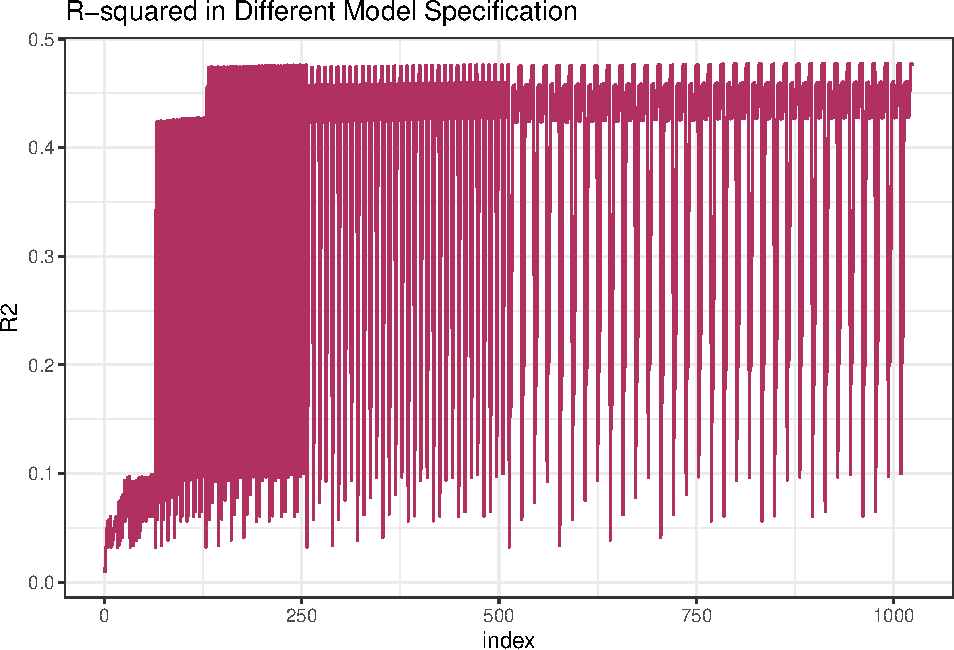
\includegraphics{hw1_files/figure-latex/unnamed-chunk-3-1.pdf}

\begin{Shaded}
\begin{Highlighting}[]
\CommentTok{# The model with the best prediction, in terms of maximizing the square of correlation, is}
\KeywordTok{which}\NormalTok{(R2 }\OperatorTok{==}\StringTok{ }\KeywordTok{max}\NormalTok{(R2))}
\end{Highlighting}
\end{Shaded}

\begin{verbatim}
## [1] 1024
\end{verbatim}

\begin{Shaded}
\begin{Highlighting}[]
\CommentTok{# which is the full model with all covariates!}
\end{Highlighting}
\end{Shaded}

\section*{2. More on racial discrimination}

Conduct two subgroup analyses:

\begin{Shaded}
\begin{Highlighting}[]
\NormalTok{resume =}\StringTok{ }\KeywordTok{read.csv}\NormalTok{(}\StringTok{"resume.csv"}\NormalTok{)}

\CommentTok{# Subsetting}
\NormalTok{male_resume <-}\StringTok{ }\NormalTok{resume }\OperatorTok
\StringTok{  }\KeywordTok{filter}\NormalTok{(sex }\OperatorTok{==}\StringTok{ "male"}\NormalTok{)}
\NormalTok{female_resume <-}\StringTok{ }\NormalTok{resume }\OperatorTok
\StringTok{  }\KeywordTok{filter}\NormalTok{(sex }\OperatorTok{==}\StringTok{ "female"}\NormalTok{)}

\NormalTok{male_table =}\StringTok{ }\KeywordTok{table}\NormalTok{(male_resume}\OperatorTok{$}\NormalTok{race, male_resume}\OperatorTok{$}\NormalTok{call)}
\NormalTok{male_table}
\end{Highlighting}
\end{Shaded}

\begin{verbatim}
##        
##           0   1
##   black 517  32
##   white 524  51
\end{verbatim}

\begin{Shaded}
\begin{Highlighting}[]
\KeywordTok{fisher.test}\NormalTok{(male_table)}
\end{Highlighting}
\end{Shaded}

\begin{verbatim}
## 
##  Fisher's Exact Test for Count Data
## 
## data:  male_table
## p-value = 0.05317
## alternative hypothesis: true odds ratio is not equal to 1
## 95 percent confidence interval:
##  0.9730068 2.5718680
## sample estimates:
## odds ratio 
##   1.571824
\end{verbatim}

\begin{Shaded}
\begin{Highlighting}[]
\NormalTok{female_table =}\StringTok{ }\KeywordTok{table}\NormalTok{(female_resume}\OperatorTok{$}\NormalTok{race, female_resume}\OperatorTok{$}\NormalTok{call)}
\NormalTok{female_table}
\end{Highlighting}
\end{Shaded}

\begin{verbatim}
##        
##            0    1
##   black 1761  125
##   white 1676  184
\end{verbatim}

\begin{Shaded}
\begin{Highlighting}[]
\KeywordTok{fisher.test}\NormalTok{(female_table)}
\end{Highlighting}
\end{Shaded}

\begin{verbatim}
## 
##  Fisher's Exact Test for Count Data
## 
## data:  female_table
## p-value = 0.0002856
## alternative hypothesis: true odds ratio is not equal to 1
## 95 percent confidence interval:
##  1.213027 1.976560
## sample estimates:
## odds ratio 
##   1.546461
\end{verbatim}

Within 95\% confident level, racial discrimination for men-employers are
insignificant, with a p-value around 0.53. Yet cincerning women
employers, the observed odds ratio is significantly different from 0
(p\textless{}0.001). Though it might be irrigorous to jump to the
conclusion that racial discrimination exists more in women's job market
(Due to ommitted variable bias.) It's a clear indicator that women are,
directly or indirectly, suffering more from the prejudice.

\section*{3. Regression adjustment in the Fisher Randomization Test}\subsubsection*{3.1 Using the residuals}

\begin{Shaded}
\begin{Highlighting}[]
\KeywordTok{library}\NormalTok{(Matching)}
\KeywordTok{data}\NormalTok{(lalonde)}
\NormalTok{result <-}\StringTok{ }\KeywordTok{lm}\NormalTok{(re78}\OperatorTok{~}\StringTok{ }\OperatorTok{-}\NormalTok{treat, }\DataTypeTok{data =}\NormalTok{ lalonde)}
\NormalTok{z <-}\StringTok{ }\NormalTok{lalonde}\OperatorTok{$}\NormalTok{treat}
\NormalTok{y <-}\StringTok{ }\NormalTok{result}\OperatorTok{$}\NormalTok{residuals}

\CommentTok{# Monte-Carlo Simulation of data}
\NormalTok{MC =}\StringTok{ }\DecValTok{10}\OperatorTok{^}\DecValTok{3}
\NormalTok{Tauhat   =}\StringTok{ }\KeywordTok{rep}\NormalTok{(}\DecValTok{0}\NormalTok{, MC)}
\NormalTok{Student  =}\StringTok{ }\KeywordTok{rep}\NormalTok{(}\DecValTok{0}\NormalTok{, MC)}
\NormalTok{Wilcox   =}\StringTok{ }\KeywordTok{rep}\NormalTok{(}\DecValTok{0}\NormalTok{, MC)}
\NormalTok{Ks       =}\StringTok{ }\KeywordTok{rep}\NormalTok{(}\DecValTok{0}\NormalTok{, MC)}
\NormalTok{tau =}\StringTok{ }\KeywordTok{t.test}\NormalTok{(y }\OperatorTok{~}\StringTok{ }\NormalTok{z, }\DataTypeTok{var.equal =} \OtherTok{TRUE}\NormalTok{)}\OperatorTok{$}\NormalTok{statistic}
\NormalTok{t =}\StringTok{ }\KeywordTok{t.test}\NormalTok{(y }\OperatorTok{~}\StringTok{ }\NormalTok{z, }\DataTypeTok{var.equal =} \OtherTok{FALSE}\NormalTok{)}\OperatorTok{$}\NormalTok{statistic}
\NormalTok{w =}\StringTok{ }\KeywordTok{wilcox.test}\NormalTok{(y }\OperatorTok{~}\StringTok{ }\NormalTok{z)}\OperatorTok{$}\NormalTok{statistic }
\NormalTok{ks =}\StringTok{ }\KeywordTok{ks.test}\NormalTok{(y[z }\OperatorTok{==}\StringTok{ }\DecValTok{1}\NormalTok{], y[z }\OperatorTok{==}\StringTok{ }\DecValTok{0}\NormalTok{])}\OperatorTok{$}\NormalTok{statistic}

\NormalTok{extreme_tau =}\StringTok{ }\DecValTok{0}
\NormalTok{extreme_t =}\StringTok{ }\DecValTok{0}
\NormalTok{extreme_w =}\StringTok{ }\DecValTok{0}
\NormalTok{extreme_ks =}\StringTok{ }\DecValTok{0}
\ControlFlowTok{for}\NormalTok{(mc }\ControlFlowTok{in} \DecValTok{1}\OperatorTok{:}\NormalTok{MC)\{}
\NormalTok{   zperm =}\StringTok{ }\KeywordTok{sample}\NormalTok{(z)}
\NormalTok{   temptau =}\StringTok{ }\KeywordTok{t.test}\NormalTok{(y }\OperatorTok{~}\StringTok{ }\NormalTok{zperm, }\DataTypeTok{var.equal =} \OtherTok{TRUE}\NormalTok{)}\OperatorTok{$}\NormalTok{statistic }
\NormalTok{   tempt =}\StringTok{ }\KeywordTok{t.test}\NormalTok{(y }\OperatorTok{~}\StringTok{ }\NormalTok{zperm, }\DataTypeTok{var.equal =} \OtherTok{FALSE}\NormalTok{)}\OperatorTok{$}\NormalTok{statistic}
\NormalTok{   tempw =}\StringTok{ }\KeywordTok{wilcox.test}\NormalTok{(y }\OperatorTok{~}\StringTok{ }\NormalTok{zperm)}\OperatorTok{$}\NormalTok{statistic }
\NormalTok{   tempks =}\StringTok{ }\KeywordTok{ks.test}\NormalTok{(y[zperm }\OperatorTok{==}\StringTok{ }\DecValTok{1}\NormalTok{], y[zperm }\OperatorTok{==}\StringTok{ }\DecValTok{0}\NormalTok{])}\OperatorTok{$}\NormalTok{statistic}
   \ControlFlowTok{if}\NormalTok{ (}\KeywordTok{abs}\NormalTok{(temptau) }\OperatorTok{>}\StringTok{ }\KeywordTok{abs}\NormalTok{(tau))\{}
\NormalTok{     extreme_tau <-}\StringTok{ }\NormalTok{extreme_tau }\OperatorTok{+}\StringTok{ }\DecValTok{1}
\NormalTok{   \}}
   \ControlFlowTok{if}\NormalTok{ (}\KeywordTok{abs}\NormalTok{(tempt) }\OperatorTok{>}\StringTok{ }\KeywordTok{abs}\NormalTok{(t))\{}
\NormalTok{     extreme_t <-}\StringTok{ }\NormalTok{extreme_t }\OperatorTok{+}\StringTok{ }\DecValTok{1}
\NormalTok{   \}}
   \ControlFlowTok{if}\NormalTok{ (}\KeywordTok{abs}\NormalTok{(tempw) }\OperatorTok{<}\StringTok{ }\KeywordTok{abs}\NormalTok{(w))\{}
\NormalTok{     extreme_w <-}\StringTok{ }\NormalTok{extreme_w }\OperatorTok{+}\StringTok{ }\DecValTok{1}
\NormalTok{   \}}
   \ControlFlowTok{if}\NormalTok{ (}\KeywordTok{abs}\NormalTok{(tempks) }\OperatorTok{>}\StringTok{ }\KeywordTok{abs}\NormalTok{(ks))\{}
\NormalTok{     extreme_ks <-}\StringTok{ }\NormalTok{extreme_ks }\OperatorTok{+}\StringTok{ }\DecValTok{1}
\NormalTok{   \}}
\NormalTok{\}}
\end{Highlighting}
\end{Shaded}

The exact p-value using tau-statistic is 0.002\\
The exact p-value using t-statistic is 0.004\\
The exact p-value using w-statistic is 0.004\\
The exact p-value using ks-statistic is 0.034\\
Those four p-values are jusified because the taking the residual in a
regression is simply a de-mean operation, subtrating the conditional
mean of the dependent variable given all the covariates other than
treatment itself. The imbalance of covariates are hence controlled after
the substraction. Almost always, it reduces the variance of our
estimation.

\subsubsection*{3.2 Using the residuals}

\begin{Shaded}
\begin{Highlighting}[]
\KeywordTok{library}\NormalTok{(Matching)}
\KeywordTok{data}\NormalTok{(lalonde)}
\NormalTok{z <-}\StringTok{ }\NormalTok{lalonde}\OperatorTok{$}\NormalTok{treat}
\NormalTok{y <-}\StringTok{ }\NormalTok{lalonde}\OperatorTok{$}\NormalTok{re78}

\CommentTok{# Monte-Carlo Simulation of data}
\NormalTok{MC =}\StringTok{ }\DecValTok{10}\OperatorTok{^}\DecValTok{3}
\NormalTok{current_coef <-}\StringTok{ }\KeywordTok{lm}\NormalTok{(re78}\OperatorTok{~}\NormalTok{., }\DataTypeTok{data =}\NormalTok{ lalonde)}\OperatorTok{$}\NormalTok{coefficients[}\StringTok{'treat'}\NormalTok{]}
\KeywordTok{lm}\NormalTok{(re78}\OperatorTok{~}\NormalTok{treat}\OperatorTok{:}\NormalTok{., }\DataTypeTok{data =}\NormalTok{ lalonde)}\OperatorTok{$}\NormalTok{coef}
\end{Highlighting}
\end{Shaded}

\begin{verbatim}
##   (Intercept)         treat     treat:age    treat:educ   treat:black 
##  4.554802e+03 -7.683564e+03  5.798286e+01  5.482296e+02 -5.904062e+02 
##    treat:hisp treat:married  treat:nodegr    treat:re74    treat:re75 
##  1.262090e+03  9.356968e+02 -7.706816e+02  2.925472e-01  1.192415e-02 
##     treat:u74     treat:u75 
##  6.920888e+03 -4.052482e+03
\end{verbatim}

\begin{Shaded}
\begin{Highlighting}[]
\NormalTok{extreme_coef <-}\StringTok{ }\DecValTok{0}
\ControlFlowTok{for}\NormalTok{(mc }\ControlFlowTok{in} \DecValTok{1}\OperatorTok{:}\NormalTok{MC)\{}
\NormalTok{  zperm =}\StringTok{ }\KeywordTok{sample}\NormalTok{(z)}
\NormalTok{  data_copy <-}\StringTok{ }\NormalTok{lalonde}
\NormalTok{  data_copy}\OperatorTok{$}\NormalTok{treat <-}\StringTok{ }\NormalTok{zperm}
\NormalTok{  coef <-}\StringTok{ }\KeywordTok{lm}\NormalTok{(re78}\OperatorTok{~}\NormalTok{., }\DataTypeTok{data =}\NormalTok{ data_copy)}\OperatorTok{$}\NormalTok{coefficients[}\StringTok{'treat'}\NormalTok{]}
  \ControlFlowTok{if}\NormalTok{ (coef }\OperatorTok{>}\StringTok{ }\NormalTok{current_coef)\{}
\NormalTok{    extreme_coef =}\StringTok{ }\NormalTok{extreme_coef }\OperatorTok{+}\StringTok{ }\DecValTok{1}
\NormalTok{  \}}
\NormalTok{\}}
\end{Highlighting}
\end{Shaded}

The exact p-value using coef-statistic is 0.005\\
It's plausible to use coefficients as our statistic because it simply
denotes the average treatment effect controlling all those covariates
constant. It can be considered as the subtraction of two regression
coefficients, indicating the difference in means. (See Lin(2013) for
detailed discussion)

\section*{5. Nonlinear causal estimands}\subsubsection*{5.1 Examples of the differents in estimands}

Example for \(\sigma_1 = \sigma_2\)

\begin{Shaded}
\begin{Highlighting}[]
\NormalTok{x <-}\StringTok{ }\KeywordTok{seq}\NormalTok{(}\DecValTok{1}\NormalTok{,}\DecValTok{10}\NormalTok{,}\DecValTok{1}\NormalTok{)}
\NormalTok{y <-}\StringTok{ }\KeywordTok{seq}\NormalTok{(}\DecValTok{2}\NormalTok{,}\DecValTok{20}\NormalTok{,}\DecValTok{2}\NormalTok{)}
\NormalTok{sigma_}\DecValTok{1}\NormalTok{ <-}\StringTok{ }\KeywordTok{median}\NormalTok{(y) }\OperatorTok{-}\StringTok{ }\KeywordTok{median}\NormalTok{(x)}
\NormalTok{sigma_}\DecValTok{2}\NormalTok{ <-}\StringTok{ }\KeywordTok{median}\NormalTok{(y}\OperatorTok{-}\NormalTok{x)}
\NormalTok{sigma_}\DecValTok{1}\OperatorTok{-}\NormalTok{sigma_}\DecValTok{2}
\end{Highlighting}
\end{Shaded}

\begin{verbatim}
## [1] 0
\end{verbatim}

\begin{Shaded}
\begin{Highlighting}[]
\CommentTok{# As long as the sign of x', y' are the same, the equation holds.}
\end{Highlighting}
\end{Shaded}

Example for \(\sigma_1 < \sigma_2\)

\begin{Shaded}
\begin{Highlighting}[]
\NormalTok{x <-}\StringTok{ }\KeywordTok{seq}\NormalTok{(}\DecValTok{1}\NormalTok{,}\DecValTok{10}\NormalTok{,}\DecValTok{1}\NormalTok{)}
\NormalTok{y[}\DecValTok{10}\NormalTok{] <-}\StringTok{ }\DecValTok{2}
\NormalTok{sigma_}\DecValTok{1}\NormalTok{ <-}\StringTok{ }\KeywordTok{median}\NormalTok{(y) }\OperatorTok{-}\StringTok{ }\KeywordTok{median}\NormalTok{(x)}
\NormalTok{sigma_}\DecValTok{2}\NormalTok{ <-}\StringTok{ }\KeywordTok{median}\NormalTok{(y}\OperatorTok{-}\NormalTok{x)}
\NormalTok{sigma_}\DecValTok{1}\OperatorTok{-}\NormalTok{sigma_}\DecValTok{2}
\end{Highlighting}
\end{Shaded}

\begin{verbatim}
## [1] -1
\end{verbatim}

Example for \(\sigma_1 > \sigma_2\)

\begin{Shaded}
\begin{Highlighting}[]
\NormalTok{y <-}\StringTok{ }\KeywordTok{seq}\NormalTok{(}\DecValTok{2}\NormalTok{,}\DecValTok{20}\NormalTok{,}\DecValTok{2}\NormalTok{)}
\NormalTok{x[}\DecValTok{10}\NormalTok{] <-}\StringTok{ }\DecValTok{1}
\NormalTok{sigma_}\DecValTok{1}\NormalTok{ <-}\StringTok{ }\KeywordTok{median}\NormalTok{(y) }\OperatorTok{-}\StringTok{ }\KeywordTok{median}\NormalTok{(x)}
\NormalTok{sigma_}\DecValTok{2}\NormalTok{ <-}\StringTok{ }\KeywordTok{median}\NormalTok{(y}\OperatorTok{-}\NormalTok{x)}
\NormalTok{sigma_}\DecValTok{1}\OperatorTok{-}\NormalTok{sigma_}\DecValTok{2}
\end{Highlighting}
\end{Shaded}

\begin{verbatim}
## [1] 1
\end{verbatim}

\subsubsection*{Find the better one}

Intuitively, the medium of differences, instead of the difference in
medians makes more sense. When we're substracting the difference of the
medians, the pre-treatment value and post-treatment value possibly will
not be attributed to the same observation. In other words, we could be
deriving a statistic based on some data that is meaningless in reality.
So in most cases, chosing the first statistic is always a safe choice.
However, it still depends on the scenario that we apply the statistic.
The following example shows that, if our goal is, say, simply to get rid
of some outliers. Given normal distributions of our original data, the
difference-in-medians statistic show a better property -- with less bias
and less variance as well.

\begin{Shaded}
\begin{Highlighting}[]
\CommentTok{# Monte-Carlo Simulation}
\CommentTok{# Assume that we already have the science table}
\CommentTok{# Also assume some normal distributions of our treatment effect}
\NormalTok{MC <-}\StringTok{ }\FloatTok{1e4}
\NormalTok{sum_of_squares_}\DecValTok{1}\NormalTok{ <-}\StringTok{ }\DecValTok{0}
\NormalTok{sum_of_squares_}\DecValTok{2}\NormalTok{ <-}\StringTok{ }\DecValTok{0}
\NormalTok{sum_}\DecValTok{1}\NormalTok{ <-}\StringTok{ }\DecValTok{0}
\NormalTok{sum_}\DecValTok{2}\NormalTok{ <-}\StringTok{ }\DecValTok{0}
\ControlFlowTok{for}\NormalTok{ (mc }\ControlFlowTok{in} \DecValTok{1}\OperatorTok{:}\NormalTok{MC)\{}
\NormalTok{  Before <-}\StringTok{ }\KeywordTok{rnorm}\NormalTok{(}\DecValTok{1000}\NormalTok{,}\DecValTok{0}\NormalTok{,}\DecValTok{1}\NormalTok{)}
\NormalTok{  treat <-}\StringTok{ }\KeywordTok{c}\NormalTok{(}\KeywordTok{rep}\NormalTok{(}\DecValTok{1}\NormalTok{,}\DecValTok{500}\NormalTok{), }\KeywordTok{rep}\NormalTok{(}\DecValTok{0}\NormalTok{,}\DecValTok{500}\NormalTok{))}
\NormalTok{  Treatment_effect <-}\StringTok{ }\KeywordTok{rnorm}\NormalTok{(}\DecValTok{1000}\NormalTok{,}\DecValTok{1}\NormalTok{,}\DecValTok{1}\NormalTok{) }\OperatorTok{*}\StringTok{ }\NormalTok{treat}
\NormalTok{  Control_effect <-}\StringTok{ }\KeywordTok{rnorm}\NormalTok{(}\DecValTok{1000}\NormalTok{,}\DecValTok{0}\NormalTok{,}\DecValTok{1}\NormalTok{) }\OperatorTok{*}\StringTok{ }\NormalTok{(}\DecValTok{1}\OperatorTok{-}\NormalTok{treat)}
\NormalTok{  After <-}\StringTok{ }\NormalTok{Before }\OperatorTok{+}\StringTok{ }\NormalTok{Treatment_effect }\OperatorTok{+}\StringTok{ }\NormalTok{Control_effect}
\NormalTok{  y <-}\StringTok{ }\NormalTok{After[}\DecValTok{1}\OperatorTok{:}\DecValTok{500}\NormalTok{]}
\NormalTok{  x <-}\StringTok{ }\NormalTok{After[}\DecValTok{501}\OperatorTok{:}\DecValTok{1000}\NormalTok{]}
\NormalTok{  sigma_}\DecValTok{1}\NormalTok{ <-}\StringTok{ }\KeywordTok{median}\NormalTok{(y) }\OperatorTok{-}\StringTok{ }\KeywordTok{median}\NormalTok{(x)}
\NormalTok{  sigma_}\DecValTok{2}\NormalTok{ <-}\StringTok{ }\KeywordTok{median}\NormalTok{(y}\OperatorTok{-}\NormalTok{x)}
\NormalTok{  sum_of_squares_}\DecValTok{1}\NormalTok{ <-}\StringTok{ }\NormalTok{sum_of_squares_}\DecValTok{1} \OperatorTok{+}\StringTok{ }\NormalTok{(sigma_}\DecValTok{1}\OperatorTok{-}\DecValTok{1}\NormalTok{)}\OperatorTok{^}\DecValTok{2}
\NormalTok{  sum_of_squares_}\DecValTok{2}\NormalTok{ <-}\StringTok{ }\NormalTok{sum_of_squares_}\DecValTok{2} \OperatorTok{+}\StringTok{ }\NormalTok{(sigma_}\DecValTok{2}\OperatorTok{-}\DecValTok{1}\NormalTok{)}\OperatorTok{^}\DecValTok{2}
\NormalTok{  sum_}\DecValTok{1}\NormalTok{ <-}\StringTok{ }\NormalTok{sum_}\DecValTok{1} \OperatorTok{+}\StringTok{ }\NormalTok{sigma_}\DecValTok{1}
\NormalTok{  sum_}\DecValTok{2}\NormalTok{ <-}\StringTok{ }\NormalTok{sum_}\DecValTok{2} \OperatorTok{+}\StringTok{ }\NormalTok{sigma_}\DecValTok{2}
\NormalTok{\}}
\end{Highlighting}
\end{Shaded}


\end{document}
